%-*-coding: utf-8-*-

\chapter{Описание предложенного алгоритма}  \label{chapter2}
В данной главе будет описан предложенный алгоритм консенсуса на основе комитета участников, проведен его анализ и доказательство,
а также возможные модификации.

\section{Схема предложенного алгоритма}
В данном разделе будет описана основная схема и краеугольные камни алгоритма.

В основе алгоритма находится комитет участников сети, 
которые принимают транзакции от \textit{клиентов} ~--- узлов, не входящих в комитет, 
и обрабатывают их.
Каждый участник комитета может быть идентифицируем некоторым образом, например, его публичным ключом, и знает идентификаторы всех остальных членов комитета.
Размер комитета равен некоторому постоянному числу $n$, которое не меняется с течением времени. 
Новый участник может присоединиться к нему, в то время как один из членов комитета должен покинуть, чтобы размер оставался равным $n$.

Комитет ответственен за корректное состояние хранилища и порядка операций, изменяющих его.
Если какой-то из участников хочет внести некоторое изменение в хранилище, остальные участники должны прийти к консенсусу, является ли оно корректным. 
Алгоритм, с помощью которого участники будут приходить к общему решению, является одной из важных частей решения.  
По сути, участники должны реализовывать задачу SMR (State Machine Replication)\cite{Schneider:1990:IFS:98163.98167}.

Таким образом, алгоритм условно можно разбить на две составляющие: алгоритм SMR в его основе и то, каким образом новые участники попадают в комитет.

\begin{figure}[!h]
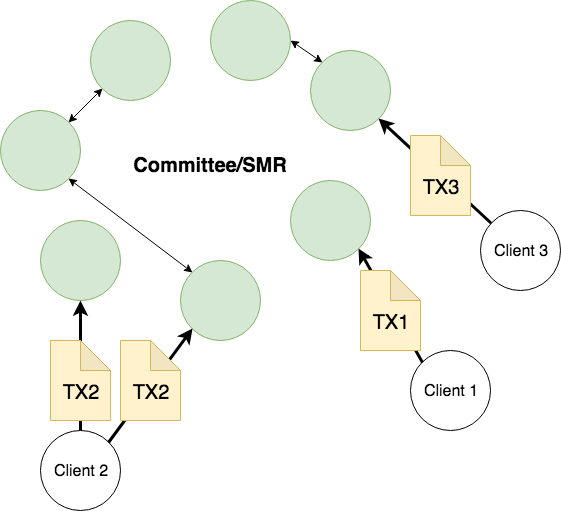
\includegraphics[scale=0.4]{Committee}
\caption{\textbf{Схематическое изображение алгоритма}}
\label{fig:committee}
\end{figure}

\section{Рассматриваемая модель}
В данном разделе мы опишем модель, в которой работает предложенный алгоритм.

В рамках данной работы мы рассматриваем \textit{инклюзивную} (permissionless) модель, в которой:
\begin{itemize}
\item множество участников алгоритма не фиксировано
\item каждый участник может начать или закончить участие в алгоритме в любое время
\item каждый участник может быть однозначно идентифицирован его публичным ключом и каждый публичный ключ однозначно определяет участника
\item одно устройство может выступать как несколько участников
\end{itemize}

Участники могут быть либо \textit{честными} (honest), либо \textit{неисправными} (faulty).  Честный участник всегда следует предписанному алгоритму, неисправный же может предпринимать действия для нарушения корректной работы алгоритма.
В рамках данной работы мы будем считать, что в комитете находится не более $f$ неисправных участников, и размер комитета $n$ равен $3f+1$.

Что касается неисправных участников, мы считаем, что они могут пытаться скомпрометировать участников комитета, пытаться подделывать их криптографические зашифрованные данные, взламывать устройство участника, и так далее. Однако, в рамках рассматриваемой модели, данные попытки занимают значительное время, что было формализовано в работе\cite{hybrid-consensus}, и носит название \textit{delayed adaptive adversary}.

Что касается модели сети, участники сети соединены в пиринговую сеть (peer-to-peer), 
то есть каждый участник поддерживает соединения с некоторыми другими участниками и обменивается с ними сообщениями. Будем считать, что любой участник может установить с любым другим участником соединение, по которому они могут обмениваться сообщениями. В следующих разделах мы разберем архитектуру сети более подробно.

В рамках данной модели сети будем считать, что отправленное сообщение может быть доставлено не более чем за время $\Delta$, которое является верхней границей на время доставки и известно заранее.
Обозначим $\delta$ как действительное время доставки сообщения от одного честного участника другому. 
Если время доставки превышает $\Delta$, считаем что участник неисправен, 
то есть $\delta \le \Delta$ для всех честных участников. 
Данная модель сети была формализована в статье Dwork \cite{Dwork:1988:CPP:42282.42283} и называется \textit{частично синхронная}(partially synchronous).

\section{Инклюзивный алгоритм SMR}
В данном разделе мы рассмотрим предложенный алгоритм, 
который является усовершенствованием алгоритма PBFT\cite{pbft} для решения задачи SMR в инклюзивной модели.
 
Так как состав комитета может меняться с течением времени, введем понятие \textit{конфигурация}, обозначающее состав комитета. Пронумеруем конфигурации, таким образом состав комитета ~--- это функция от его номера $c$, которую мы будем обозначать как $C(c)$. 
 
Один из участников в конфигурации является \textit{лидером}, который управляет алгоритмом SMR. 
Остальные участники конфигурации являются \textit{последователями}, которые проверяют и подтверждают действия лидера. Все честные последователи знают, какой участник является лидером.

Лидер в конфигурации может меняться с течением времени, при этом конфигурация может оставаться неизменной. Пронумеруем участников в конфигурации $c$ от нуля до $n-1$, тогда лидером с номером $v$ будет участник $L(c, v)$:
  \[
  L(c, v)=\Bigg\{ 
  \begin{array}{ll}
  0, v = 0\\
  \mathcal{H}(c, v) \mod n, v > 0 
  \end{array}
  \]

\subsection{Устойчивое состояние} \label{steady-state}
В данном разделе будет показано, как участники комитета приходят к консенсусу при постоянных $c$ и $v$. Данное состояние неизменности $c$ и $v$ называется \textit{устойчивым состоянием} (steady state).

Прежде всего, введем понятие \textit{лога примененных изменений} ~--- это индексируемый с нуля список, где нулевой элемент в списке ~--- первое примененное изменение, первый элемент ~--- следующее, и так далее. У каждого участника комитета имеется своя копия лога изменений, обозначим ее как $Log$, которые были применены к его локальной копии хранилища. \textit{Текущим слотом} будем называть $s$ равную длине $Log$. 
В ходе алгоритма, участники сообщения пытаются \textit{заполнить} текущий слот одинаковым сообщением, перейдя к следующему слоту.

Помимо лога и текущего слота каждый участник комитета хранит следующие данные:
\begin{itemize}
\item номер текущей конфигурации $c$ и номер лидера $v$
\item список публичных ключей всех участников конфигурации с номером $c$ 
\item собственный секретный ключ
\item состояние, которое может обновляться инкрементально
\end{itemize}

Прежде чем перейти к описанию, введем следующее обозначение:
\[ \langle tag, a_1, a_2, ... a_n \rangle_X \] будем обозначать сообщение с тегом $tag$ и полями $a_1$, $a_2$..., $a_n$, подписанное секретным ключом участника $X$. Тег в данном случае ~--- это некоторая строка, которая отличает различные типы сообщений и делает невозможным переиспользование одного сообщения в качестве другого с точно такими же полями.

Теперь опишем как новое изменение попадает в лог участника комитета.

Пусть комитет находится в конфигурации с номером $c$ и лидером с номером $v$. 
Пусть лидер $L$ ($L = L(c, v)$) честный и хочет внести изменение $d$ в логи всех участников комитета. Алгоритм происходит в три раунда.

\textbf{Раунд 1. Предложение}. Лидер отправляет всем участникам конфигурации сообщение 
\[ \langle Propose, c, v, s, d \rangle_L \]

1.1 Каждый честный последователь $F$, получив сообщение, проверяет следующее:
\begin{itemize}
\item $c$, $v$ и $s$ из сообщения равны локальным значениям
\item подпись сообщения корректна и соответствует публичному ключу $L$
\item $proposed_{c, v, s}$ еще не занято другим $\hat d$
\item валидно ли изменение $d$ и возможно ли применить его к состоянию
\end{itemize}

Если все вышеперечисленные проверки выполнились, $F$ присваивает $proposed_{c, v, s} := d$, в противном случае, $F$ игнорирует присланное сообщение. 
\vspace{10pt}

\textbf{Раунд 2. Подготовка}. Каждый честный последователь $F$, для которого выполнились все предыдущие проверки, отправляет лидеру $L$ сообщение 
\[ \langle Prepare, c, v, s, d \rangle_F \]

2.1 Лидер $L$, получив Prepare-сообщение, проверяет, что
\begin{itemize}
\item $c$, $v$ и $s$ из сообщения равны локальным значениям
\item подпись сообщения корректна и соответствует публичному ключу $F$
\item $d$ соответствует сообщению $Propose$ для $s$, отправленному им в предыдущем раунде
\end{itemize}
Если какая-то из проверок не выполнилась, лидер игнорирует присланное сообщение. 

2.2 Лидер дожидается $2f+1$ сообщений $Prepare$ (включая свое собственное) с одинаковыми значением $c$, $v$, $s$ и $d$ и формирует \textit{сертификат согласия} (Acceptance certificate), обозначим его как $\mathcal{P}$. Данный сертификат является гарантией того, что как минимум $2f+1$ участников (среди которых как минимум $f+1$ честных) пришли к согласию, что текущий слот $s$ должен быть заполнен изменением $d$.

Пока для простоты будем считать, что $\mathcal{P}$ ~--- это кортеж
$$(c, v, s, d, \sigma_1, \sigma_2, ..., \sigma_{2f+1})$$
где $Prepare$ ~--- это тег, а $\sigma_i$ ~--- подпись $Prepare$ сообщения $i$-го приславшего участника (включая самого лидера). 
В последующих разделах, формирование сертификата $\mathcal{P}$ будет проанализировано и улучшено.

2.3 После этого лидер отправляет всем последователям  $\mathcal{P}$

2.4 Каждый честный последователь $F$, получив сертификат, проверяет следующее:
\begin{itemize}
\item $c$, $v$, $s$ из сообщения равны локальным значениям
\item $proposed_{c, v, s} = d$
\item все подписи в $\mathcal{P}$ корректны
\end{itemize}
\vspace{10pt}

Если все проверки выполнились, то участник запоминает данный сертификат в $acceptance_s := \mathcal{P}$.
\vspace{10pt}

\textbf{Раунд 3. Применение}.
Каждый честный последователь $F$, для которого выполнились все предыдущие проверки, отправляет лидеру $L$ сообщение 
\[ \langle Commit, c, v, s, d \rangle_F \]

3.1 Лидер $L$, получив $Commit$-сообщение, проверяет его аналогично шагу 2.1.
Если какая-то из проверок не выполнилась ~--- лидер игнорирует присланное сообщение. 

3.2 Лидер дожидается $2f+1$ сообщений $Commit$ (включая свое собственное) с одинаковыми значением $c$, $v$, $s$ и $d$ и формирует \textit{сертификат применения} (Commit certificate), обозначим его как $\mathcal{C}$.
$$\mathcal{C}=(c, v, s, d, \sigma_1, \sigma_2, ..., \sigma_{2f+1})$$

3.3 После этого лидер отправляет всем последователям $\mathcal{C}$

3.4 Каждый честный последователь $F$, получив сертификат, проверяет его аналогично шагу 2.4.
Если все проверки выполнились ~--- последователь добавляет изменение $d$ в свой лог и применяет изменение $d$ к своему локальному состоянию.

3.5 После этого, участник комитета уведомляет клиентов о новом изменении, отправляя им:
 \[ \langle Notify, \mathcal{C} \rangle_M \]

Следует отметить, что лидер следует всем шагам алгоритма действуя и как лидер, и как последователь. За исключением того, что он не отправляет сообщения самому себе.

Будем называть сертификат \textit{корректным}, если все подписи в нем корректны.
Стоит обратить внимание, что вообще говоря два последователя $F_1$ и $F_2$ могут получить разные корректные сертификаты согласия $\mathcal{P}_1$ и $\mathcal{P}_2$ и/или применения $\mathcal{C}_1$ и $\mathcal{C}_2$ с одинаковыми $c, v, s, d$, однако, это не нарушает корректность алгоритма, при условии что сертификаты корректны.
То есть лидер может дождаться более чем $2f+1$ $Prepare$/$Commit$ сообщения и сформировать каждому последователю корректный сертификат, отличный от других.

Также, если лидер отправляет последователю сертификат для $s$, в то время как последователь уже имеет корректный сертификат для $s$, то последователь игнорирует присланный.

\subsection{Реконфигурация} \label{reconfig}
В данном разделе будет описано, как комитет переходит в новую конфигурацию, то есть как обновляется состав комитета. Данный шаг называется реконфигурация ~--- то есть изменение конфигурации.

Схема реконфигурации состоит в том, что \textit{майнеры} ~--- участники сети, которые хотят вступить в комитет, совершают работу по решению некоторого \textit{пазла}. После того как решение найдено, майнер публикует данное решение в комитет, каждый участник комитета проверяет его, и после нескольких раундов сообщений между участником и майнером, участник сообщает майнеру, что решение корректно и участник готов принять его в комитет.
После чего, текущий лидер комитета предлагает изменение, которое добавляет майнера в комитет.

Формально, решение пазла ~--- это некоторое число $\phi$, что:
$$\mathcal{H}(puzzle^c, pk, \phi) < target$$
где $\mathcal{H}$ ~--- криптографически стойкая хэш-функция, $puzzle^c$ ~--- это некоторая величина, зависящая от $c$, называемая \textit{пазлом}, $pk$ ~--- публичный ключ майнера, $target$ ~--- некоторое число, которое задает сложность вычисления.

Другими словами, майнеры выполняют доказательство выполненной работы (PoW), подобно тому, как это делается в Bitcoin.  Число $target$ выбирается так, чтобы поиск числа $\phi$ примерно занимал некоторое время $D$, намного большее $\Delta$. Скажем, $D$ равное 10 минутам, как и в Bitcoin подойдет.  $target$ также меняется со временем, и зависит от частоты нахождения предыдущих значений $PoW$, более подробно с тем, как выбирается $target$ можно познакомиться в оригинальной статье \cite{nakamoto}.
Как формируется число $puzzle_c$ будет рассказано далее в этом разделе. Сосредоточимся более подробно на том, как майнер добавляется в комитет.

Майнера, который нашел число $\phi$, будем называть \textit{кандидатом}.
Прежде всего, каждый участник комитета для конфигурации $c$ хранит множество известных ему кандидатов $Q$.
\vspace{10pt}

Итак, после того, как майнер $W$ нашел число $\phi$, он отправляет всем участникам комитета сообщение
 \[ \langle Candidate, c, puzzle^c, pk, \phi \rangle_W \]
 
Участник $M$, получивший данное сообщение, выполняет следующую последовательность шагов:

1.1 Берет эксклюзивную блокировку $B$ на чтение данных. То есть откладывает обработку сообщения от лидера $L(c, v)$ до тех пор, пока блокировка не будет отпущена. 

1.2 Проверяет, что выполняется все из следующего:
\begin{itemize}
\item корректность подписи $W$ 
\item корректность решения пазла, то есть что $\mathcal{H}(puzzle^c, pk, \phi) < target$
\item $c$ из сообщения равно локальному значению
\end{itemize}

1.3 Засекает таймер $T$ на $5\Delta$ и отправляют кандидату $W$ сообщение:
 \[ \langle Status, c, \hat{\mathcal{C}}, pk \rangle_M \]
где $c$, $v$~--- локальные значения, $\hat{\mathcal{C}}$~--- последний сертификат применения, $pk$~--- публичный ключ $W$.
\vspace{10pt}

После того как $W$ получает $2f+1$ корректно подписанных $Status$ сообщений с ожидаемым $c$, он проверяет все $\hat{\mathcal{C}}_i$ и вычисляет $s^{*}=max(s_1, s_2,..., s_{2f+1})+2$, где $s_i$~--- слоты из $\hat{\mathcal{C}}_i$ из $Status$ сообщений.
Далее отправляет всем участникам запрос на подтверждение слота:
 \[ \langle ReserveSlot, c, s^{*} \rangle_W \]
 
\noindent Участник $M$, получивший это сообщение, проверяет:
\begin{itemize}
\item корректность подписи W
\item $c$ равно локальному значению
\item $proposed_{c, v, s^{*}}$ еще не заполнено никаким изменением $d'$
\end{itemize} 
После чего отправляет в ответ $W$:
 \[ \langle ConfirmSlot, c, s^{*}, pk \rangle_M \]
где $pk$~--- публичный ключ $W$.
\vspace{10pt}

После получения $2f+1$ корректно подписанных $Confirm$, с одинаковыми значениями $c$, $v$ и $s^{*}$,
формирует и отправляет всем участникам комитета \textit{сертификат кандидата} $\mathcal{S}$:

$$\mathcal{S}=(c, s^{*}, pk, \sigma_1, \sigma_2,..., \sigma_{2f+1})$$
$\sigma_i$ ~--- подписи $ConfirmSlot$ сообщений.
\vspace{10pt}

Участник $M$, получивший сертификат $\mathcal{S}$, выполняет шаги : 

2.1 Проверяет подписи $ConfirmSlot$ сообщений $\sigma_i$.

2.2 Проверяет, что $c$ из $\mathcal{S}$ равно локальному, а $s^{*} \ge s + 2$

2.3 Отправляет данный сертификат всем остальным участникам комитета.

2.4 Добавляет $\mathcal{S}$ в $Q$.

2.5 Снимает блокировку на ресурсы $B$.

Если кандидат не успевает прислать сертификат $\mathcal{S}$ до истечения таймера $T$, блокировка $B$ снимается.

Данная процедура во-первых гарантирует, что либо все честные участники, либо ни одного (в зависимости от честности действий кандидата) узнают о новом кандидате, а во-вторых что как минимум $f+1$ честных участников придут к консенсусу о $s^{*}$.

После того, как все честные участники, в том числе и лидер $L(c, v)$, узнали о кандидатах, претендующих на добавление в комитет, участники ожидают от лидера, что в скором времени лидер предложит изменение, которое изменит конфигурацию комитета. А именно, каждый раз, когда участник получает $Propose$ сообщение, помимо проверок описанных в  разделе \ref{leader-change}, он проверяет, что данное сообщение $Propose$ содержит тех, и только тех кандидатов из $Q$, для которых выполняется $s^{*} = s$, где $s$~--- слот из $Propose$ сообщения. Если же это условие не выполняется, участник игнорирует данное $Propose$ сообщение.

Изменение реконфигурации $d_{rec}$ формально описывается следующим образом:
$$d_{rec}=((puzzle^c_1, pk_1, \phi_1, \sigma_1), (puzzle^c_2, pk_2, \phi_2, \sigma_2),...,(puzzle^c_k, pk_k, \phi_k, \sigma_k))$$
где $k$~--- количество кандидатов, $\sigma_i$~--- подпись $Candidate$ сообщения.

Как только $d_{rec}$ будет применено и попадет в лог применений, необходимо произвести реконфигурацию.
Реконфигурация задается функцией $\Phi$ из изменения реконфигурации в список кандидатов. Данная функция определяет каких кандидатов и в каком порядке необходимо добавить в комитет, следовательно, столько же самых давних участников должны покинуть его. Для простоты рассмотрим $\Phi$, которая возвращает кандидата, у которого решение пазла является наименьшим, то есть $\mathcal{H}(puzzle^c_i, pk_i, \phi_i)$ наименьше, а при равенстве, выберем c наименьшим $pk_i$.

Итак, после того как участник $M$ получил сертификат применения $d_{rec}$~--- $\mathcal{C}$, он выполняет следующие шаги:

3.1 Отправляет и участникам, и клиентам
 \[ \langle Notify, \mathcal{C} \rangle_M \]

3.2 Проверяет, является ли он самым давним участником, покидает комитет и перестает выполнять дальнейшие шаги. 

В противном случае выполняет последующие шаги алгоритма:

3.3 Вызывает процедуру актуализации лога применений (которая будет описана в разделе \ref{act_log})

3.4 Добавляет $d_{rec}$ в лог применений

3.5 Вычисляет $pk=\Phi(d_{rec})$

3.6 Добавляет кандидата $pk$ в список участников комитета и убирает самого старого из списка

3.7 Увеличивает $c$ на один и обнуляет $v$

3.8 Очищает $Q := \{\}$

3.9 Запускает процедуру актуализации лога применений для сертификата $d_{rec}$, которая описана в разделе \ref{act_log}.

Таким образом, кандидат становится нулевым участником, и тем самым новым лидером.

\vspace{10pt}

После того, как кандидат $W$ получит $f+1$ корректное $Notify$ сообщение, он начинает действовать как лидер комитета. В данный момент реконфигурация считается проведенной успешно и комитет переходит в новое устойчивое состояние.

После того, как майнер получает $f+1$ $Notify$ сообщение, он формирует
$puzzle^{c+1}=(\sigma_1, \sigma_2,..., \sigma_{f+1})$
где $\sigma_i$~--- подписи $Notify$ сообщений. После чего может начинать работу над новым пазлом.

\subsection{Смена лидера} \label{leader-change}
В данном разделе будет описано, как участники комитета переходят к лидеру с номером $v+1$, если текущий лидер препятствует прогрессу системы. Прежде всего опишем, как последователь обнаруживает \textit{отсутствие прогресса}.

Будем считать, что лидер производит изменения довольно часто. В следующих разделах будет пояснено, почему данное предположение корректно.

После очередного применения некоторого изменения $d$ или смены лидера последователь $M$ запускает таймер на время $5\Delta$ ~--- за это время честный лидер должен успеть провести 3 раунда описанных выше, и последователь должен получить следующее изменение.
Данная величина получена из следующих соображений, что последователи обмениваются с лидером пятью сообщениями, и так как мы считаем, что в рамках данной модели сообщение, отправленное честным участником не должно идти дольше времени $\Delta$, данная процедура не должна занять больше $5\Delta$.

После того, как последователь $M$ обнаружил отсутствие прогресса, то есть состояние, при котором текущий лидер не предложил новое изменение за время $5\Delta$, последователь переходит в \textit{состояние смены лидера}.
Результат выхода из этого состояния будет следующее устойчивое состояние с новыми $c$ и $v$.
Цель описанного далее процесса~--- сформировать сертификат \textit{устойчивого состояния}:
$$\mathcal{W}=(c, v', s^{*}, \mathcal{C}^{*}, \mathcal{P}^{*}, Q^{*}, \sigma_{L(c, v')}, \varkappa_1, \varkappa_2,..., \varkappa_{2f+1})$$

Данный сертификат содержит значения $c, v', s$, на которых участники согласовываются, переходя в новое устойчивое состояние, а также о последних имеющихся у участников сертификатах согласия и множествах кандидатов.

Итак, после того, как участник $M$ перешел в состояние смены лидера, он проделывает следующее:

1.1. Перестает принимать сообщения с тегом отличным от $LeaderChange$ и $NewLeader$

1.2. Отправляет сообщение новому лидеру $L(c, v+1)$:
\[ \langle LeaderChange, c, v+1,  \hat{\mathcal{C}}, \hat{\mathcal{P}}, Q \rangle_M \]
где $\hat{\mathcal{C}}$ и $\hat{\mathcal{P}}$~--- последнний сертификат применения и согласия, полученный $M$, $Q$~--- известные $M$ кандидаты.

1.3. Засекает таймер на $6\Delta$.

1.4. Если таймер истек, $M$ не перешел в новое устойчивое состояние, то он повторяет шаги 2 и 3 для следующего лидера $v+2$. Данный шаг будет повторяться до тех пор, пока $M$ не окажется в устойчивом состоянии.
\vspace{10pt}

После того, как новый лидер $L(c, v')$ получит $2f+1$ корректно подписанных сообщений $LeaderChange$ с одинаковыми $c$ и $v'$  (включая свое) далее формирует отправляет всем участникам:
\[ \langle Election, c, v', \hat{\mathcal{C}}_1,...,\hat{\mathcal{C}}_{2f+1}, \hat{\mathcal{P}}_1,...,\hat{\mathcal{P}}_{2f+1}, Q_1,..., Q_{2f+1}, \sigma_1,..., \sigma_{2f+1}\rangle_{L(c, v')} \]

Получив данное сообщение, участник $M$:
\begin{itemize}
\item подпись $Election$ корректна
\item значение $c$ из сертификата совпадает с локальным
\item $v'$ строго больше локального $v$
\item корректность всех $\hat{\mathcal{P}}_i$ и $\hat{\mathcal{C}}_i$
\item корректность всех подписей $\sigma_i$
\end{itemize}
Если хотя бы одна из проверок не выполнилась, $M$ игнорирует сообщение, иначе выполняет следующее:

2.1. Находит сертификат $\mathcal{C}^{*}$, в котором значение слота наибольшее и равно $s^{*}$, аналогично $\mathcal{P}^{*}$ вместе с  $s_P^{*}$, причем если существует несколько сертификатов согласия с $s_P^{*}$, участник выбирает с наибольшим значением $(c, v)$, а также вычисляет $Q^{*} = \bigcup\limits_{i=1}^{2f+1} Q_i$.

2.2. Отправляет лидеру в ответ
\[ \langle Vote, c, v', s^{*}, \mathcal{C}^{*}, \mathcal{P}^{*}, Q^{*}, \sigma_{L(c, v')} \rangle_M \]
где $\sigma_{L(c, v')}$~--- подпись сообщения $Election$.
\vspace{10pt}

Получив $2f+1$ $Vote$ сообщений с одинаковыми $c, v', \mathcal{C}^{*}, \mathcal{P}^{*}, Q^{*}, \sigma_{L(c, v')}$, новый лидер $L(c, v')$ формирует и отправляет сертификат \textit{устойчивого состояния}:
$$\mathcal{W}=(c, v', s^{*}, \mathcal{C}^{*}, \mathcal{P}^{*}, Q^{*}, \sigma_{L(c, v')}, \varkappa_1, \varkappa_2,..., \varkappa_{2f+1})$$
$\varkappa_i$ ~--- это подпись $Vote$ сообщения $i$-го приславшего участника.

После того как участник $M$ получил сертификат, он проверяет следующее:
\begin{itemize}
\item значение $c$ из сертификата совпадает с локальным
\item $v'$ строго больше локального $v$
\item слот $s^{*}$ соответствует $\mathcal{C}^{*}$
\item корректность всех $\mathcal{C}^{*}$ и $\mathcal{P}^{*}$
\item корректность всех подписей $\varkappa_i$
\end{itemize}
Если хотя бы одна из проверок не выполнилась, $M$ игнорирует сообщение. В противном случае:

3.1. Отправляет всем участникам $\mathcal{W}$

3.2. Проводит процедуру актуализации лога применений с $\mathcal{C}^{*}$

3.3. Обновляет $Q := Q^{*}$.

3.4. Обновляет $v := v'$ и тем самым \textit{принимает} нового лидера.

3.5. Обновляет $acceptance_{s_P^{*}} := \hat{\mathcal{P}}^{*}$

6. В случае если $s_P^{*}=s^{*}+1$, отправляет
\[ \langle Commit, c, v', s_P^{*}, d^{*} \rangle_F \]
где $d^{*}$ изменение из $\mathcal{P}^{*}$ и дожидается сертификата применения от $L(c, v')$, после чего участник переходит в новое устойчивое состояние, присваивая $leaderChange := False$, иначе по истечению таймера переходит к смене лидера.

3.7. Если условие в шаге 6 не выполнилось, то есть $s^{*}=s_P^{*}$, переходит в новое устойчивое состояние после шага 6, присваивая $leaderChange := False$.

Стоит обратить внимание, что участник $M$ может уже иметь сертификат применения для $s_P^{*}$, $d^{*}$, однако в случае выполнения  шага 6, он все равно отправляет $Commit$ сообщение.

Процедура смены лидера несет две цели: достигнуть консенсуса о новом лидере, а также актуализировать логи всех честных участников, устраняя отставание, которое мог создать предыдущий лидер.

В следующей главе будет доказано, что либо $s_P^{*}=s^{*}$, либо $s_P^{*}=s^{*}+1$, то есть либо сертификат согласия соответствует сертификату применения, либо сертификат согласия соответствует предложенному предыдущим лидером изменению.

\subsection{Процедура актуализации лога применений} \label{act_log}
Процедура актуализации лога применений необходима для устранения отставания участника комитета.
Она принимает на вход текущий слот участника $s$ и сертификат согласия или применения, имеющийся у участника.

Обозначим $s$ текущий слот участника комитета $M$, а $s_k$ номер слота из сертификата. Если $s \le s_k-1$, тогда $M$ отправляет любым $f+1$ участникам из сертификата 
\[ \langle RequestCommits, s, s_k-1 \rangle_M \]
тем самым запрашивая изменения соответствующие слотам $s, s+1,..., s_k-1$

Участник $M'$, получивший данное сообщение и имеющий сертификаты применения для соответствующих слотов, отправляет их в ответ
\[ \langle ReponseCommits, \mathcal{C}_s, \mathcal{C}_{s+1},...,\mathcal{C}_{s_k-1} \rangle_{M'} \]

Получив их $M$ проверяет корректность каждого из них и применяет изменения к состоянию, добавляя их после этого в лог применений. Таким образом процедура гарантирует, что в лог применений будет заполнен по слот $s_k-1$ включительно.

\section{Отправка транзакций в комитет}
В данной главе будет описано, как клиенты отправляют транзакции в комитет.

Пусть некоторый клиент $A$ сформировал транзакцию $tx$. Далее он отправляет в комитет сообщение
\[ \langle Send, tx \rangle_A \]
после того, как участник $M$ получил сообщение:

1. Проверяет корректность транзакции

2. Отправляет $tx$ лидеру

3. Добавляет $tx$ в свой \textit{мемпул} (mempool)~--- список известных ему транзакций. 

4. Рассчитывает, до какого слота $\hat{s}$ транзакция должна попасть в лог применения

5. Отправляет клиенту сообщение
\[ \langle Promise, tx, \hat{s} \rangle_M \]
получая $2f+1$ $Promise$ сообщение, клиент формирует \textit{сертификат обещания}:
$$Pr=(Promise, tx,  \hat{s}_1,  \hat{s}_2,..., \hat{s}_{2f+1}, \sigma_1, \sigma_2,...,\sigma_{2f+1})$$

Если клиент хочет гарантировать, что его транзакция обязательно добавится в лог применения, он может следить за $Notify$ сообщениями. Обозначим $s_{tx}=max(\hat{s}_1,  \hat{s}_2,..., \hat{s}_{2f+1})$. Если клиент получает $Notify$ сообщение с корректным сертификатом для слота $s \le s_{tx}$ и изменения, в котором содержится транзакция $tx$, участник может считать, что его транзакция успешно обработана. В противном случае, если он получил $Notify$ сообщение для слота $s_{tx}$ и изменения, в котором не содержится $tx$, то клиент может сообщить о нечестности лидера, отправив $2f+1$ участникам сообщение
\[ \langle Report, \mathcal{C}, Pr \rangle_A \]
где $\mathcal{C}$~--- сертификат применения из $Notify$ сообщения.

Участник, получив это сообщение, проверяет корректность $\mathcal{C}$ и $Pr$, запускает процедуру актуализации лога применения, далее проверяет, что $max(\hat{s}_1,  \hat{s}_2,..., \hat{s}_{2f+1}) \le s$ и переходит в состояние смены лидера.

\subsection{Виртуальные участники}
В разделе \ref{reconfig} описано, как новые участники присоединяются к комитету. Как уже было отмечено описано выше, участники комитета идентифицируются своими публичными ключами. До сих пор мы неявно предполагали, что в комитете не может быть два одинаковых публичных ключа. Однако, одно физическое устройство может сгенерировать несколько секретных ключей с соответствующими публичными, более того, член комитета может сделать то же самое, и таким образом одному \textit{реальному} участнику комитета будет соответствовать несколько \textit{виртуальных}. В рамках данной работы ограничение на количество неисправных участников накладывается именно на виртуальных.

С одной стороны, если реальный участник выйдет из строя или его устройство будет скомпроментировано, то все его виртуальные участники выйдут из строя или станут нечестными.  Однако, данное ограничение является естественным в инклюзивной модели, так как нет способа каким-либо образом идентифицировать участника, в отличии от эксклюзивной модели, где идентификация может быть произведена централизовано.

С другой стороны, данное ограничение играет на руку, так как ограничение на долю владения честными участниками некоторого процента вычислительной мощности вычисляется из суммарной вычислительной мощности во всей системе, а не только устройств вне комитета. Другими словами, если бы существовал способ запретить участникам комитета снова присоединяться к нему, используя другого виртуального участника, тогда была бы возможна такая ситуация, когда в комитете состояли участники с довольно большим процентом вычислительной мощности от общего в системе, а среди устройств вне комитета процент владения мощностью честных и нечестных участников примерно равен или даже нечестные участники превосходят честных. В данном случае нечестные участники присоединялись бы к комитету в большем количестве, нежели честные. В текущей же модели, с большей вероятностью к комитету присоединиться виртуальный участник уже существующего реального участника комитета, и невозможно будет создать угрозу безопасности системы.

\section{Стартовый запуск}
В предыдущих разделах было описано, как комитет приходит к согласию о порядке транзакций, а также как он пополняется новыми участниками, однако, чему равно $C_1$? То есть каков состав комитета при старте системы. Необходимо некоторым образом сформировать состав первого комитета.

Одно из решений состоит в том, чтобы реализовать упрощенную версию алгоритма Nakamoto consensus и дождаться, пока $n$ участников решат $n$ пазлов и выпустят $n$ блоков с решениями, которые образуют цепочку. Каждый пазл будет зависеть от всех уже найденных решений. После чего, все $n$ участников нашедших решения пазлов образуют начальную конфигурацию $C_1$, первый из нашедших является лидером.
Однако, у такого решения есть следующие недостатки: длительность формирования первого комитета зависит от осведомленности и заинтересованности общественности, а также, участники могут использовать эгоистичный майнинг\cite{DBLP:journals/corr/EyalS13}, так как пазл зависит только от уже найденных решений. Чтобы избежать этого, они могут пописать найденное решение, что повысит энтропию следующего пазла. Но нечестные участники могут отказаться подписывать. Данные проблемы приводят нас к следующему более гибкому решению.

Второе решение состоит в том, чтобы изначально сформировать комитет из доверенных участников. Так, количество реальных участников $n'$ может быть значительно меньше $n$, однако каждый из них будет иметь около $\frac{n}{n'}$ виртуальных. У данного решения тоже есть недостаток, в том что при отказе одного реального устройства комитет покидают $\frac{n}{n'}$ виртуальных. Таким образом, в первое время, до тех пор пока не произойдет порядка $n$ реконфигураций, система должна быть довольно стабильна и отзывчива.
С другой стороны, в данном случае с самого старта система может функционировать и устойчива к эгоистичному майнингу.

\section{Микроблоки}
Рассмотрим, что может использоваться в качестве изменения $d$. Первая приходящая в голову идея~--- использовать транзакции пользователей. Однако, предложенный алгоритм частично-синхронен, в частности он не обрабатывает другие изменения, пока не добавит в лог обрабатываемое в данный момент изменение. Таким образом, обработка транзакции индивидуально ухудшит пропускную способность.

Поэтому возникает другая идея~--- группировать несколько транзакций и создавать микроблок. И лидер выпускает микроблоки~--- блоки содержащие все транзакции из его мемпула. 

Получая $Propose$ сообщение с микроблоком, участник проверяет, что все транзакции могут быть последовательно добавлены в хранилище.
И после того как микроблок попадает в лог применений участника, участник убирает из собственного мемпула все транзакции содержащиеся в блоке. Таким образом, участник всегда хранит некоторый корректный список транзакций, которы	e могут быть последовательно применены к хранилищу.

Чтобы избежать смены лидера, текущий лидер должен с некоторой периодичностью выпускать изменения. Предполагается, что, если его мемпул пуст~--- лидер выпустит пустой микроблок.

%\section{Уменьшение размера сертификата}